\section{结论}
% ============================================================
% Frame: 好控制变量
% ============================================================
\begin{frame}[allowframebreaks]{好控制变量}

  % --- 好控制变量1: 共同原因X ---
  \begin{columns}[c]
    \begin{column}{0.55\textwidth}
      \begin{block}{1. D和Y的共同原因X}
        X同时影响D和Y，不控制会导致遗漏变量偏误。控制X后，分块内部处理状态近似随机，选择性偏误被消除。

        \medskip
        \textbf{应该控制。}
      \end{block}
    \end{column}
    \begin{column}{0.4\textwidth}
      \centering
      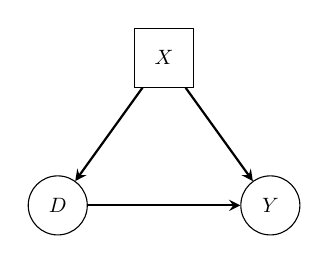
\begin{tikzpicture}[scale=0.75, every node/.style={scale=0.75}]
        \tikzstyle{circ} = [draw, circle, minimum size=1cm, align=center, inner sep=1pt]
        \tikzstyle{sq} = [draw, rectangle, minimum size=1cm, align=center, inner sep=1pt]
        \node[sq] (X) at (1, 2.5) {$X$};
        \node[circ] (D) at (-0.8, 0) {$D$};
        \node[circ] (Y) at (2.8, 0) {$Y$};
        \draw[->, >=stealth, thick] (X) -- (D);
        \draw[->, >=stealth, thick] (X) -- (Y);
        \draw[->, >=stealth, thick] (D) -- (Y);
      \end{tikzpicture}

      {\footnotesize \fbox{方框} $=$ 好控制变量}
    \end{column}
  \end{columns}

  \framebreak

  % --- 好控制变量2: 代理变量G ---
  \begin{columns}[c]
    \begin{column}{0.55\textwidth}
      \begin{block}{2. 遗漏变量$\varepsilon$的代理变量G}
        如果$\varepsilon$无法直接观测，但G是$\varepsilon$影响D的机制变量（$\varepsilon \to G \to D$），控制G可间接剥离D和$\varepsilon$的相关性。

        \medskip
        \textbf{应该控制。}
      \end{block}
    \end{column}
    \begin{column}{0.4\textwidth}
      \centering
      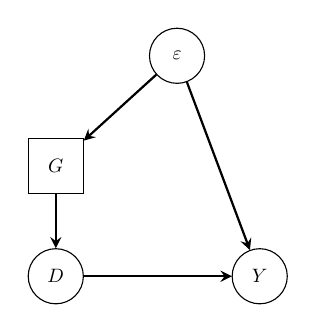
\begin{tikzpicture}[scale=0.7, every node/.style={scale=0.7}]
        \tikzstyle{circ} = [draw, circle, minimum size=1cm, align=center, inner sep=1pt]
        \tikzstyle{sq} = [draw, rectangle, minimum size=1cm, align=center, inner sep=1pt]
        \node[circ] (eps) at (1, 4) {$\varepsilon$};
        \node[sq] (G) at (-1.2, 2) {$G$};
        \node[circ] (D) at (-1.2, 0) {$D$};
        \node[circ] (Y) at (2.5, 0) {$Y$};
        \draw[->, >=stealth, thick] (eps) -- (G);
        \draw[->, >=stealth, thick] (eps) -- (Y);
        \draw[->, >=stealth, thick] (G) -- (D);
        \draw[->, >=stealth, thick] (D) -- (Y);
      \end{tikzpicture}
    \end{column}
  \end{columns}

  \framebreak

  % --- 好控制变量3: Y的原因P ---
  \begin{columns}[c]
    \begin{column}{0.55\textwidth}
      \begin{block}{3. Y的原因变量P，且与D无关}
        控制P能吸收误差项方差，降低标准误，提高统计功效。因P与D无关，不会吸收处理变量的变异性。

        \medskip
        纯粹提高精度，不影响因果识别。
      \end{block}
    \end{column}
    \begin{column}{0.4\textwidth}
      \centering
      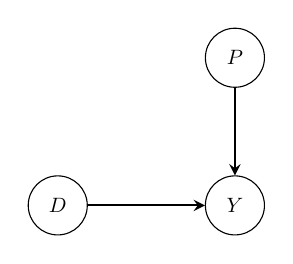
\begin{tikzpicture}[scale=0.75, every node/.style={scale=0.75}]
        \tikzstyle{circ} = [draw, circle, minimum size=1cm, align=center, inner sep=1pt]
        \node[circ] (D) at (-1, 0) {$D$};
        \node[circ] (Y) at (2, 0) {$Y$};
        \node[circ] (P) at (2, 2.5) {$P$};
        \draw[->, >=stealth, thick] (D) -- (Y);
        \draw[->, >=stealth, thick] (P) -- (Y);
      \end{tikzpicture}
    \end{column}
  \end{columns}

\end{frame}

% ============================================================
% Frame: 坏控制变量
% ============================================================
\begin{frame}[allowframebreaks]{坏控制变量}

  % --- 坏控制变量1: 对撞变量Q ---
  \begin{columns}[c]
    \begin{column}{0.55\textwidth}
      \begin{alertblock}{1. 对撞变量（Collider）Q}
        Q是D和u（影响Y的因素）的共同结果。不控制时D和u不相关；控制Q后，D和u人为产生相关性，凭空引入选择性偏误。

        \medskip
        \textbf{不应该控制。}
      \end{alertblock}
    \end{column}
    \begin{column}{0.4\textwidth}
      \centering
      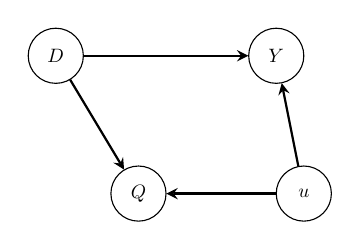
\begin{tikzpicture}[scale=0.7, every node/.style={scale=0.7}]
        \tikzstyle{circ} = [draw, circle, minimum size=1cm, align=center, inner sep=1pt]
        \node[circ] (D) at (-1.5, 2.5) {$D$};
        \node[circ] (Y) at (2.5, 2.5) {$Y$};
        \node[circ] (Q) at (0, 0) {$Q$};
        \node[circ] (u) at (3, 0) {$u$};
        \draw[->, >=stealth, thick] (D) -- (Y);
        \draw[->, >=stealth, thick] (D) -- (Q);
        \draw[->, >=stealth, thick] (u) -- (Q);
        \draw[->, >=stealth, thick] (u) -- (Y);
      \end{tikzpicture}

      {\footnotesize 圆圈 $=$ 坏控制变量}
    \end{column}
  \end{columns}

  \framebreak

  % --- 坏控制变量2a: 中介变量M（简单情形）---
  \begin{columns}[c]
    \begin{column}{0.55\textwidth}
      \begin{alertblock}{2a. 中介变量（Mediator）W}
        $D \to W \to Y$ 路径上的变量。控制W会阻断间接效应路径，只剩直接效应，低估甚至反转总因果效应的方向。

        \medskip
        \textbf{不应该控制——过度控制。}
      \end{alertblock}
    \end{column}
    \begin{column}{0.4\textwidth}
      \centering
      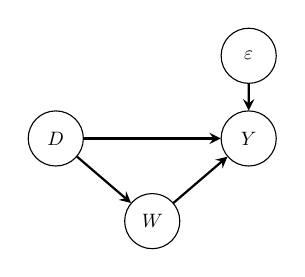
\begin{tikzpicture}[scale=0.7, every node/.style={scale=0.7}]
        \tikzstyle{circ} = [draw, circle, minimum size=1cm, align=center, inner sep=1pt]
        \node[circ] (eps) at (2.5, 3) {$\varepsilon$};
        \node[circ] (D) at (-1, 1.5) {$D$};
        \node[circ] (Y) at (2.5, 1.5) {$Y$};
        \node[circ] (W) at (0.75, 0) {$W$};
        \draw[->, >=stealth, thick] (D) -- (Y);
        \draw[->, >=stealth, thick] (D) -- (W);
        \draw[->, >=stealth, thick] (W) -- (Y);
        \draw[->, >=stealth, thick] (eps) -- (Y);
      \end{tikzpicture}
    \end{column}
  \end{columns}

  \framebreak

  % --- 坏控制变量2b: 中介 + 对撞（复合情形）---
  \begin{columns}[c]
    \begin{column}{0.55\textwidth}
      \begin{alertblock}{2b. 中介变量同时也是对撞变量}
        现实中几乎一定存在不可观测因素u同时影响W和Y。此时W同时是中介和对撞变量，控制它会同时产生过度控制和对撞偏误。

        \medskip
        \textbf{双重危害。}
      \end{alertblock}
    \end{column}
    \begin{column}{0.4\textwidth}
      \centering
    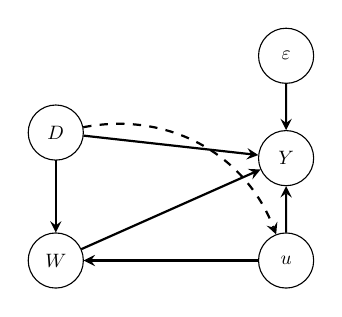
\begin{tikzpicture}[scale=0.65, every node/.style={scale=0.7}]
  \tikzstyle{circ} = [draw, circle, minimum size=1cm, align=center, inner sep=1pt]
  \node[circ] (eps) at (3, 3.5) {$\varepsilon$};
  \node[circ] (D) at (-1.5, 2) {$D$};
  \node[circ] (Y) at (3, 1.5) {$Y$};
  \node[circ] (W) at (-1.5, -0.5) {$W$};
  \node[circ] (u) at (3, -0.5) {$u$};
  \draw[->, >=stealth, thick] (D) -- (Y);
  \draw[->, >=stealth, thick] (D) -- (W);
  \draw[->, >=stealth, thick] (W) -- (Y);
  \draw[->, >=stealth, thick] (u) -- (W);
  \draw[->, >=stealth, thick] (u) -- (Y);
  \draw[->, >=stealth, thick] (eps) -- (Y);
  \draw[->, >=stealth, thick, dashed] (D) to[bend left=40] (u);
\end{tikzpicture}
    \end{column}
  \end{columns}

  \framebreak

  % --- 坏控制变量3: Y的结果变量R ---
  \begin{columns}[c]
    \begin{column}{0.55\textwidth}
      \begin{alertblock}{3. Y的结果变量R}
        控制R会将潜在结果不可比的群体放在一起比较，产生选择性偏误。

        \medskip
        \textbf{不应该控制。}
      \end{alertblock}
    \end{column}
    \begin{column}{0.4\textwidth}
      \centering
      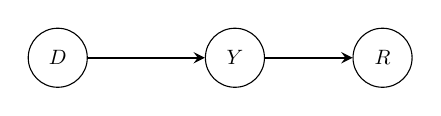
\begin{tikzpicture}[scale=0.75, every node/.style={scale=0.75}]
        \tikzstyle{circ} = [draw, circle, minimum size=1cm, align=center, inner sep=1pt]
        \node[circ] (D) at (-1.5, 0) {$D$};
        \node[circ] (Y) at (1.5, 0) {$Y$};
        \node[circ] (R) at (4, 0) {$R$};
        \draw[->, >=stealth, thick] (D) -- (Y);
        \draw[->, >=stealth, thick] (Y) -- (R);
      \end{tikzpicture}
    \end{column}
  \end{columns}

  \framebreak

  % --- 坏控制变量4: D的原因W ---
\begin{columns}[c]
    \begin{column}{0.55\textwidth}
      \begin{alertblock}{4. D的原因变量W（统计推断层面）}
        控制W会大量吸收处理变量D的变异性，导致标准误显著增大、统计功效下降。虽不引入偏误，但让估计变得非常不精确。

        \medskip
        \textbf{不建议控制。}
      \end{alertblock}
    \end{column}
    \begin{column}{0.4\textwidth}
      \centering
    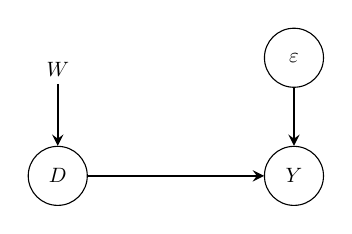
\begin{tikzpicture}[scale=0.75, every node/.style={scale=0.75}]
  \tikzstyle{circ} = [draw, circle, minimum size=1cm, align=center, inner sep=1pt]
  \node[circ] (eps) at (2.5, 2) {$\varepsilon$};
  \node (W) at (-1.5, 1.8) {$W$};
  \node[circ] (D) at (-1.5, 0) {$D$};
  \node[circ] (Y) at (2.5, 0) {$Y$};
  \draw[->, >=stealth, thick] (W) -- (D);
  \draw[->, >=stealth, thick] (D) -- (Y);
  \draw[->, >=stealth, thick] (eps) -- (Y);
\end{tikzpicture}
    \end{column}
  \end{columns}

\end{frame}

% ============================================================
% Frame: 总览图
% ============================================================

\begin{frame}{控制变量分类总览}

  \begin{center}
  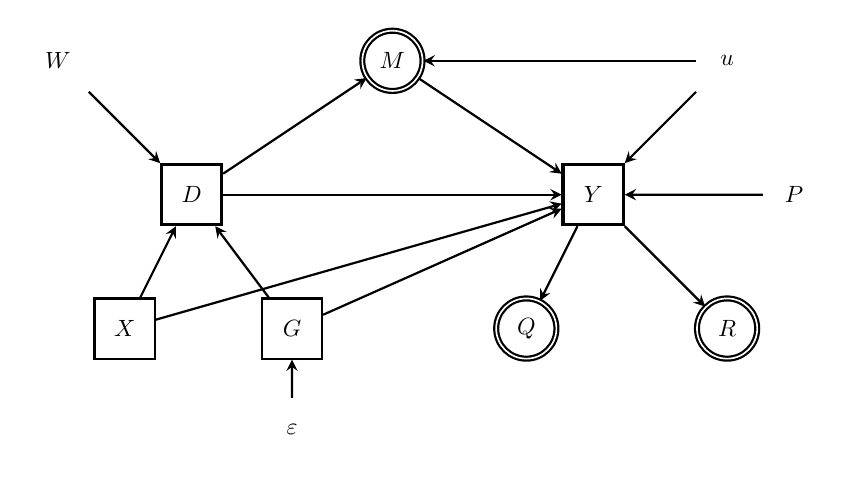
\begin{tikzpicture}[scale=0.85, every node/.style={scale=0.85},
    >=stealth, thick,
    good/.style={draw, rectangle, minimum size=0.9cm, align=center, inner sep=3pt},
    bad/.style={draw, circle, minimum size=0.9cm, align=center, double},
    core/.style={draw, rectangle, minimum size=0.9cm, align=center, inner sep=3pt, line width=1.2pt},
    plain/.style={minimum size=0.9cm, align=center}]

    % === 第一行: W, M, u, P (y=4) ===
    \node[plain] (W) at (-5, 4) {$W$};
    \node[bad]   (M) at (0, 4)  {$M$};
    \node[plain] (u) at (5, 4)  {$u$};

    % === 第二行: D, Y, P (y=2) ===
    \node[core]  (D) at (-3, 2) {$D$};
    \node[core]  (Y) at (3, 2)  {$Y$};
    \node[plain] (P) at (6, 2)  {$P$};

    % === 第三行: X, G, Q, R (y=0) ===
    \node[good]  (X) at (-4, 0) {$X$};
    \node[good]  (G) at (-1.5, 0) {$G$};
    \node[bad]   (Q) at (2, 0)  {$Q$};
    \node[bad]   (R) at (5, 0)  {$R$};

    % === 第四行: epsilon (y=-1.5) ===
    \node[plain] (eps) at (-1.5, -1.5) {$\varepsilon$};

    % === 连线 ===
    % W → D
    \draw[->] (W) -- (D);

    % D → Y (核心因果路径)
    \draw[->] (D) -- (Y);

    % D → M, M → Y (中介路径)
    \draw[->] (D) -- (M);
    \draw[->] (M) -- (Y);

    % u → M, u → Y
    \draw[->] (u) -- (M);
    \draw[->] (u) -- (Y);

    % P → Y
    \draw[->] (P) -- (Y);

    % Y → Q, Y → R
    \draw[->] (Y) -- (Q);
    \draw[->] (Y) -- (R);

    % X → D, X → Y
    \draw[->] (X) -- (D);
    \draw[->] (X) -- (Y);

    % G → D, G → Y
    \draw[->] (G) -- (D);
    \draw[->] (G) -- (Y);

    % eps → G
    \draw[->] (eps) -- (G);

  \end{tikzpicture}
  \end{center}

  \vspace{0.3em}
  \centering
  \footnotesize
  \fbox{方框} $=$ 因果识别的好控制变量 \qquad
  \tikz\draw[double, thick] (0,0) circle (0.3cm); $=$ 坏控制变量

\end{frame}